\documentclass[conference]{IEEEtran}
\IEEEoverridecommandlockouts
% The preceding line is only needed to identify funding in the first footnote. If that is unneeded, please comment it out.
\usepackage{cite}
\usepackage{amsmath,amssymb,amsfonts}
\usepackage{algorithmic}
\usepackage{graphicx}
\usepackage{braket}
\usepackage{textcomp}
\usepackage{siunitx}
\usepackage{xcolor}
\def\BibTeX{{\rm B\kern-.05em{\sc i\kern-.025em b}\kern-.08em
    T\kern-.1667em\lower.7ex\hbox{E}\kern-.125emX}}

\newcommand{\iu}{{i\mkern1mu}}

\begin{document}

\title{Quantum Computing}

\author{\IEEEauthorblockN{Andrei Tumbar}
\IEEEauthorblockA{\textit{Computer Engineering} \\
Rochester Institute of Technology\\
Rochester, United States \\
at1777@rit.edu}
\and
\IEEEauthorblockN{Justin Shaytar}
\IEEEauthorblockA{\textit{Computer Engineering} \\
Rochester Institute of Technology\\
Rochester, United States \\
jas7650@rit.edu}
}

\maketitle

\begin{abstract}
Quantum Computing has been shown to exhibit computational capabilities that far surpass those of conventional computing for certain classes of problems. Researchers in Quantum Computing (QC) have been searching for better ways to stabilize quantum bit coherance which has a high susceptibility to electromagnetic and thermal noise. QC varies greatly from the operation of the classical computation design which made this field very attractive to mathmatician and physicists. This paper will discuss the driving theory behind QC as well as modern implementations and applications.
\end{abstract}

\begin{IEEEkeywords}
Quantum Computing, optimization, entanglement, adiabatic computing, qubit
\end{IEEEkeywords}

\section{Introduction}

Classical computing relies on transistor logic to drive discrete functions represented with 2-state systems. While Quantum Computing is able to represent the same functions, it is also able to take advantage of the probabilistic nature of quantum mechanics to drive more complex functionality. The idea was initially pioneered by Richard Feynman while trying to model the interaction of quantum particles of increasing counts \cite{b1}. Attempting to simulate many particle interactions with a conventional computer quickly becomes unreasonable even for modern supercomputers as the number of variables grow exponentially. QCs does not suffer from this deficiency as the state of the quantum system will rise exponentially with the number of qubits in the system. Feynman's approach to simulating physics could be expanded to simulate any large physical system with the known characteristic behaviour of a quantum system \cite{b2}. A universal computer clearly fits this criteria as it is itself a physical system.

Though the field of QC is quite promising, the actual implementation of a reliable quantum system is far from ready. \cite{b1} theorizes that the number of qubits needed to implement a fully fault-tolerant universal computer is over 1 million. As of late 2021, the largest quantum computer is IBM's 127-qubit Eagle processor (disputed) \cite{b3}. The likely use of quantum computers in the near future could be synonymous with the relationship between an ASIC or co-processor and a conventional processor. A smaller number of qubits controlled by a fixed quantum gate circuit could solve select problems to greatly accelerate computation intensive algorithms. Keeping logic intensive algorithms in the domain of classical computing will likely stay constant for the considerable future. 

\section{Birth of Quantum Computing}

To describe why Richard Feynman was interested in the simulation of many quantum particles interacting with each other, it is best to first introduce classical wave mechanics and interference. The double slit experiment is the example that first comes to mind. Here, a single beam of light is shined through a surface with two small slits. One might expect the light to shine directly through and illuminate the slits on the screen located behind.

\begin{figure}[htbp]
\centerline{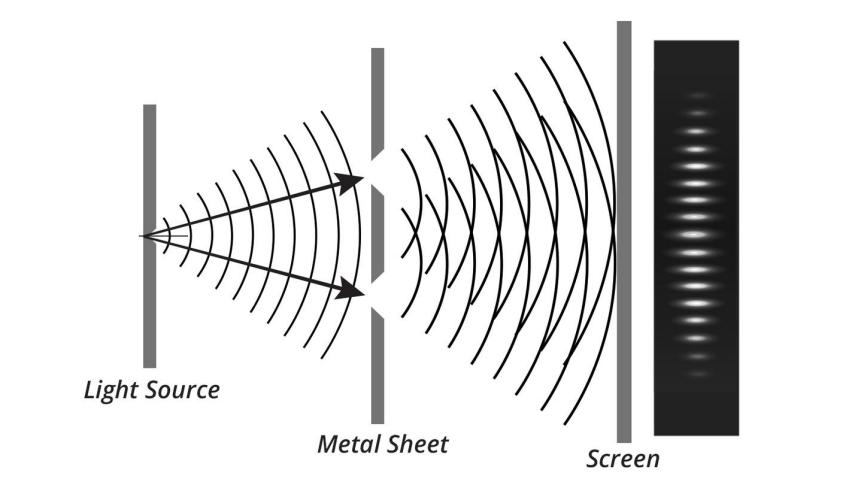
\includegraphics[width=8cm]{double_slit_wave}}
\caption{Wave double slit showing wave interference.}
\label{wave_slit}
\end{figure}

Figure \ref{wave_slit} shows the basic setup of the double wave experiment. Looking at Figure \ref{wave_slit}, we can see that the expected behaviour is not exhibited. When the light shines through each of the slits, the resultant waves will interfere with each other to produce a fringe pattern. Because of the cone propagation pattern of a wave, this result is intuitive. The interaction between waves is well understood and can easily be modelled. The next logical experiment to perform is to use a particle beam instead of light. The interaction between individual particles, in this case electrons, was thought to be similar to that of large particles interacting with each other. Once again, expected behaviour of firing electrons through the double slit would be to see two slits on the opposite screen. To the surprise of many physicists, a fringe pattern similar to that of the wave double slit experiment was seen \cite{b4}. The implications are of course quite significant: quantum particles behave in a more complex fashion that what was previously thought. We now know that the behaviour of a single quantum non-realistic particle can be described by Schr\"{o}dinger's equation:

\begin{equation}
i\hbar {\frac {\partial }{\partial t}}\Psi (x,t)=\left[-{\frac {\hbar ^{2}}{2m}}{\frac {\partial ^{2}}{\partial x^{2}}}+V(x,t)\right]\Psi (x,t)
\label{schrodeq}
\end{equation}

\begin{figure}[htbp]
\centerline{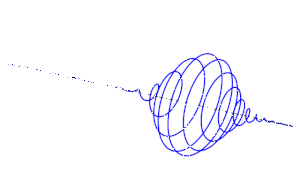
\includegraphics[width=8cm]{schrodinger}}
\caption{Complex plot of wave function that satisfies Schr\"{o}dinger's equation.}
\label{schrod}
\end{figure}

Equation \ref{schrodeq} is a wave function that assigns a complex number to each point $x$ at each time $t$. Figure \ref{schrod} visualizes this equation at a constant time $t$. A single particle traveling in a single dimension is relatively simple to simulate using discrete numerical methods. Adding more quantum particles to the system will increase the complexity exponentially. Feynman quickly concluded that classical computation could not be scaled to accommodate this sort of problem. The complexity would far outweigh the capabilities of even the most modern conventional supercomputers. Feynman theorized the use of a ``quantum computer" in which the simulation of the quantum system could be modelled by quantum particles themselves \cite{b4}. The idea here was to use single particles to represent the state of a system and could therefore contrain the operating physics of the computer to that of which we are trying to simulate.

\section{Quantum Information Theory}

Classical computation relies upon on a discrete 2-state system. Normally we represent logical state by a voltage level (high or low). QC operates within the $\mathbb{C}^2$ space. States are respresented with two complex scalars in Dirac's Braket notion \cite{b1}:
\begin{equation*}
\ket{\psi} = \alpha\ket{0} + \beta\ket{1} = \begin{pmatrix}
	\alpha\\
	\beta
	\end{pmatrix}
\end{equation*}

\begin{figure}[htbp]
\centerline{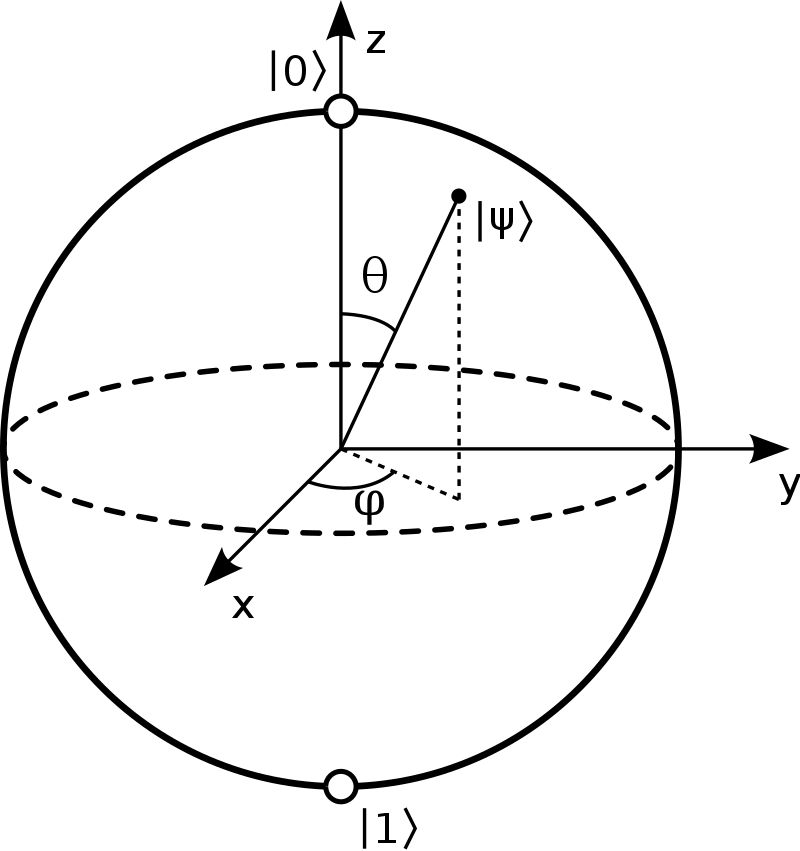
\includegraphics[width=4cm]{bloch_sphere}}
\caption{Bloch sphere representing $\mathbb{C}^2$ space with $|\alpha|^2 + |\beta|^2=1$ constraint.}
\label{bloch_sphere}
\end{figure}

$\alpha$ and $\beta$ are both complex scalars satisfying the normalization criteria $|\alpha|^2 + |\beta|^2=1$. This state vector is known as a quantum bit or more commonly: qubit. Because of its normalization property, all possible qubit states can be represented with a three dimensional sphere with $r=1$ known as the Bloch Sphere (Figure \ref{bloch_sphere}). Qubit states must lie on the outer shell of the sphere. A qubit must be measured to determine its state. Measuring a qubit will result in either a $\ket{0}$ with a probability $|\alpha|^2$ and $\ket{1}$ with probability $|\beta|^2$. Once measured, a qubit will stay in measured state which will effect the entire quantum system. So even though the qubit is a number in $\mathbb{C}^2$, we may only extract a single bit of information during measurement \cite{b5}. For example, take a qubit with state $\begin{pmatrix}
	\frac{1}{\sqrt{2}}\\
	\frac{1}{\sqrt{2}}
	\end{pmatrix}$, when measured the result is of course either $\ket{0}$ or $\ket{1}$. Both of outcomes have a probablity of $\frac{1}{2}$.

The most important take-away of a qubit is that every state is a sum of probabilities that the qubit will collapse into $\ket{0}$ or $\ket{1}$ upon measurement. If measured again, there is a 100\% probability it will be measured with the same value. Measurement will in turn effect the state of the system and should therefore be differed until the end. In fact, a classical bit can be thought of as a qubit when the values are exactly $\ket{0}$ and $\ket{1}$ and therefore have $100 \%$ chance of collapsing into their respective classical states. By this token, if you want to be able to represent a qubit with classical bits, you would need infinitely many as the possible states of a qubit are uncountably infinite. Simulation of quantum computing using classical computing therefore approximates qubit representation using a limited number of classical bits and fixed precision numbers.

\subsection{Quantum Gates}

Being able to transform a qubit's state is crucial to provide a form of ``quantum programming". A quantum gate (QG) works similarly to a conventional digital gate with the distinction that gates are transformations that occur in-place and must be reversible. A quantum gate must be a unitary operator meaning that it will not change the norm of the state vector. This is required to hold the normalization criteria of the collapsable state probabilities $||\hat{\psi}|| = |\alpha|^2 + |\beta|^2 = 1$. A quantum circuit will consist of some network of quantum gates and a set of measurement gates at the end of the circuit to extract the classical bits out of the quantum state. Measurement of the system must be performed at the end as entangled qubits (discussed later) will collapse together if one of the entangled pair is measured. This means that measuring a single qubit can affect the greater quantum computer depending on the configuration of the circuitry.

The classic example of a unary quantum gate is the set of Pauli gates. The three Pauli gates, $X$, $Y$ and $Z$ will rotate a qubit by $\pi$ radians across their respective axis. Single bit gates can be represented as a $2 \times 2$ matrix transform.

\begin{align*}
X = \begin{pmatrix}
	0 & 1\\
	1 & 0
\end{pmatrix} \Rightarrow X \ket{0} &= \ket{1} && \text{Pauli X gate}\\
X\ket{1} &= \ket{0}\\
Y = \begin{pmatrix}
	0 & -\iu\\
	\iu & 0
\end{pmatrix} \Rightarrow Y \ket{0} &= \iu\ket{1} && \text{Pauli Y gate}\\
Y\ket{1} &= -\iu\ket{0}\\
Z = \begin{pmatrix}
	1 & 0\\
	0 & -1
\end{pmatrix} \Rightarrow Z \ket{0} &= \ket{0} && \text{Pauli Z gate}\\
Z\ket{1} &= -\ket{1}
\end{align*}

Pauli X gate performs quantum logical not by rotating $\pi$ radians about X-axis. We can see that the other two Pauli gates, will perform rotation operations that will change the phase of the qubit state. Pauli Z is special in that it will only rotate the phase and not the logical state. This will exhibit a special property as the state vector may be changed but the bit extracted after a measurement will remain unaffected. The examples shown in the equation above simply show the cases when the qubit is $\ket{0}$ or $\ket{1}$, of course there are infinitely more states that these gates will operate on.\cite{b5}

\begin{figure}[htbp]
\centerline{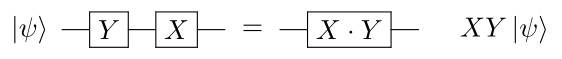
\includegraphics[width=8cm]{serially_pauli_xy.png}}
\caption{Two gates applied in order $Y$, $X$.}
\label{serial_pauli}
\end{figure}

The Pauli gates are very simple as they only operate on a single qubit. There are of course more complex gates that can operate on multi-bit inputs such as the Toffoli which operates on three bits $\ket{a,b,c} \rightarrow\ket{a,b,c \oplus (a \land b)}$. Quantum gates may also be ``serially wired" to produce combinations of transformations.

\subsection{Special Gates}

Before we continue to the next section of this paper, we must first introduce two important gates that will be used for entanglement and teleportation. These two gates are the Hadamard and controlled not gate (CNOT).

\begin{align*}
H = \frac{1}{\sqrt{2}}\begin{pmatrix}
	1 & 1\\
	1 & -1
\end{pmatrix} \Rightarrow H \ket{0} &= \begin{pmatrix}
	\frac{1}{\sqrt{2}}\\
	\frac{1}{\sqrt{2}}
\end{pmatrix} && \text{Hadamard gate}
\end{align*}

Notice how the Hadamard gate is able to take a $\ket{0}$ qubit and transform it into a state where the qubit has an equal probablity of collapsing into any of the two $\ket{0}$ or $\ket{1}$ states. The CNOT gate will work different from the other gates so far discussed in that instead of operating on a single bit, it will operate on two bits. Here is the ``truth" table if we are talking about classical bit inputs:

\begin{table}[htbp]
\caption{CNOT binary operation}
\begin{center}
\begin{tabular}{|c|c||c|c|}
\hline
\multicolumn{2}{|c||}{\textbf{Inputs}} & \multicolumn{2}{c|}{\textbf{Outputs}}\\\hline
0 & 0 & 0 & 0 \\\hline
0 & 1 & 0 & 0 \\\hline
1 & 0 & 1 & 1 \\\hline
1 & 1 & 1 & 0 \\\hline
\end{tabular}
\label{tab:cnot}
\end{center}
\end{table}

As you can see from Table \ref{tab:cnot}, the logical properties of the gate will be $F\ket{a|b} = \ket{a|a \oplus b}$. This of course can be represented as the matrix:

\begin{align*}
\text{CNOT} = \begin{pmatrix}
	1 & 0 & 0 & 0\\
	0 & 1 & 0 & 0\\
	0 & 0 & 0 & 1\\
	0 & 0 & 1 & 0
\end{pmatrix}
\end{align*}

The CNOT gate operates on two bits. One bit is called the control bit while the other is simply the input. This gate will have the same functionality as the XOR gate in classical computing when the inputs to the function are either $\ket{0}$ or $\ket{1}$. The distinction between the CNOT and XOR gate is that one of the outputs to the gate is the input. This is common for all quantum gates as one of the requirements of a quantum gate must be that given an output, its unique input must be discernible.

\section{Entanglement \& Teleportation}

In this section we will introduce the idea of quantum entanglement and then show how quantum teleportation operates. Many scientific and engineering papers will attempt to simplify a topic by drawing an analogy that can be easily conceptualized by a reader. The issue with in quantum physics is that there is no analogy that can be drawn to easily explain phenomenon that drive the computation. For this reason, we will simply be looking at the mathematics and ``believe" the results.

The first step is to look at the effect that a CNOT gate has on two qubits with arbitrary states. We will define two qubits with arbitrary states $\ket{q_0}$ and $\ket{q_1}$.

\begin{align*}
\ket{q_0} = \begin{pmatrix}x\\y\end{pmatrix}\;\;
\ket{q_1} = \begin{pmatrix}\alpha\\\beta\end{pmatrix}
\end{align*}

The next step is to create a 2-qubit state using the tensor product of the two state vectors.

\begin{align*}
\ket{q_0} \otimes \ket{q_1} &= \begin{pmatrix}
x \cdot \begin{pmatrix}\alpha\\\beta\end{pmatrix}\\
y \cdot \begin{pmatrix}\alpha\\\beta\end{pmatrix}
\end{pmatrix}
= \begin{pmatrix}x\alpha\\x\beta\\y\alpha\\y\beta\end{pmatrix}
\end{align*}

Now we can apply a CNOT gate to the state of the system by using its matrix transform.

\begin{align*}
\text{CNOT} \times (\ket{q_0} \otimes \ket{q_1}) &= \begin{pmatrix}
	1 & 0 & 0 & 0\\
	0 & 1 & 0 & 0\\
	0 & 0 & 0 & 1\\
	0 & 0 & 1 & 0
\end{pmatrix} \begin{pmatrix}x\alpha\\x\beta\\y\alpha\\y\beta\end{pmatrix} = \begin{pmatrix}x\alpha\\x\beta\\y\beta\\y\alpha\end{pmatrix}
\end{align*}

Multiplying this CNOT matrix had the expected result of swapping the last two rows. With the above math finished, we will try to tensor factor the resultant state vector into the individual qubit states.

\begin{align*}
\begin{pmatrix} x\alpha \\ x\beta \\ y\beta \\ y\alpha \end{pmatrix} &= \ket{q_0'} \otimes \ket{q_1'}
= \begin{pmatrix}
x \cdot \begin{pmatrix}\alpha\\\beta\end{pmatrix}\\
y \cdot \begin{pmatrix}\beta\\\alpha\end{pmatrix}
\end{pmatrix}\\
\end{align*}

This as far as we can go during the factoring process as there is no solution to yield the tensor product $\ket{q_0'} \otimes \ket{q_1'}$. This means there is no generalized way to described the state of the system with each individual bit. Lets try placing known inputs into the CNOT gate.

\begin{gather*}
\ket{q_0} = \ket{1} = \begin{pmatrix}0\\1\end{pmatrix}\\
\ket{q_1} = \ket{0} = \begin{pmatrix}1\\0\end{pmatrix}\\
\text{CNOT}(\ket{q_0} \otimes \ket{q_1}) =
\begin{pmatrix}x\alpha\\x\beta\\y\beta\\y\alpha\end{pmatrix} =
\begin{pmatrix}0\\0\\0\\1\end{pmatrix} = \begin{pmatrix}x'\alpha'\\x'\beta'\\y'\alpha'\\y'\beta'\end{pmatrix}
\end{gather*}

Again, we want to express the solution vector as a tensor product of two qubits. The resultant qubits, $\ket{q_0'}$ and $\ket{q_1'}$, are represented by $\begin{pmatrix}x'\\y'\end{pmatrix}$ and $\begin{pmatrix}\alpha'\\\beta'\end{pmatrix}$. To tensor factor and find the state of the system, we can solve a system of equations:

\begin{gather*}
x'\alpha' = 0 \;\;\;\; x'\beta' = 0\\
y'\alpha' = 0 \;\;\;\; y'\beta' = 1\\
x' = 0, \; y' = 1 \Rightarrow \ket{q_0'} = \ket{1} \\
\alpha' = 0, \; \beta' = 1 \Rightarrow \ket{q_1'} = \ket{1}
\end{gather*}

The solution state matches our prediction shown in Table \ref{tab:cnot} -- $\text{CNOT}(\ket{10}) = \ket{11}$. Now here's where things become interesting. Lets choose a qubit states that are not part of the ``logical set" ($\ket{0}$ and $\ket{1}$). In this case we choose $\frac{\ket{0} + \ket{1}}{\sqrt{2}}$ and $\ket{0}$. The first state is of course the output of a Hadamard gate given an input of $\ket{0}$.

\begin{gather*}
\ket{q_0} = \frac{1}{\sqrt{2}}\begin{pmatrix}1\\1\end{pmatrix}\\
\ket{q_1} = \ket{0} = \begin{pmatrix}1\\0\end{pmatrix}\\
\text{CNOT}(\ket{q_0} \otimes \ket{q_1}) =
\begin{pmatrix}x\alpha\\x\beta\\y\beta\\y\alpha\end{pmatrix} =
\frac{1}{\sqrt{2}}\begin{pmatrix}1\\0\\0\\1\end{pmatrix} = \begin{pmatrix}x'\alpha'\\x'\beta'\\y'\alpha'\\y'\beta'\end{pmatrix}
\end{gather*}

Notice how we set up the problem in the exact same way as previously with $\ket{1}$ and $\ket{0}$ as inputs. Now we attempt to solve the system of equations the same way:

\begin{gather*}
x'\alpha' = \frac{1}{\sqrt{2}} \;\;\;\; x'\beta' = 0\\
y'\alpha' = 0 \;\;\;\; y'\beta' = \frac{1}{\sqrt{2}}
\end{gather*}

We can see this system of equations is impossible to solve. To satisfy the second equation, either $x'$ or $\beta'$ must be $0$. However to satisfy the first and fourth equations this cannot be true. What this means is that the state of the quantum system $\ket{q_0'q_1'}$ cannot be described as a collection of separate bits. This is called an entangled state and can be described in Dirac's notation with $\frac{\ket{00}+\ket{11}}{\sqrt{2}}$. Entanglement will form the basis of quantum gate computing and is also required to understand quantum teleportation.

\begin{figure}[htbp]
\centerline{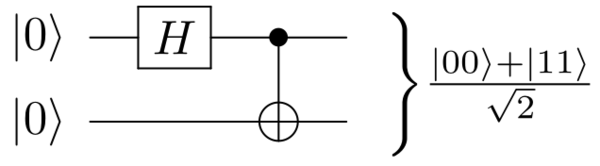
\includegraphics[width=8cm]{entanglement_circuit.png}}
\caption{Quantum Entanglement demonstrated using a circuit of a Hadamard and CNOT gate.}
\label{entanglement}
\end{figure}

Figure \ref{entanglement} shows the quantum circuit used to create an entangled pair. We know from the Hadamard circuit described in the previous section that $H\ket{0} = \ket{q_0}$ where $\ket{q_0}$ is the input to the example we just discussed. The second gate shown in the figure is a CNOT gate. One of the most important features of quantum entanglement is that once one of the qubits is measured, the other qubit will collapse to the same state \cite{b8}. Not only will they collapse to the same state, the measurement will apply to both at the exact same time regardless of physical distance between the two particles.

\subsection{Quantum Teleportation}

A 2013 paper \cite{b7} cited a practical expirement where two qubits were entangled and physically separated by great distance by firing one of the entangled qubits into space via a laser. \cite{b7} showed that the qubits remained entangled and would exhibit the same properties regardless of the distance. This brings us to quantum teleportation. Simple entanglement cannot transmit any information. When we collapse one qubit the other qubit will also collapse however we have not gained any new information. Put another way, if two people, Bob and Alice each hold a single half of an entangled particle. When Bob measures his particle and collapses the qubit, Alice's qubit will also collapse. Technically there was no information that was sent to Alice, the collapse of the state was simply coordinated between the two particles. Bob cannot send an arbitrary value to Alice with a simple entangled pair.

Unlike with the entanglement circuit, we will instead start with the quantum teleportation circuit and show how it implements teleportation.

\begin{figure}[htbp]
\centerline{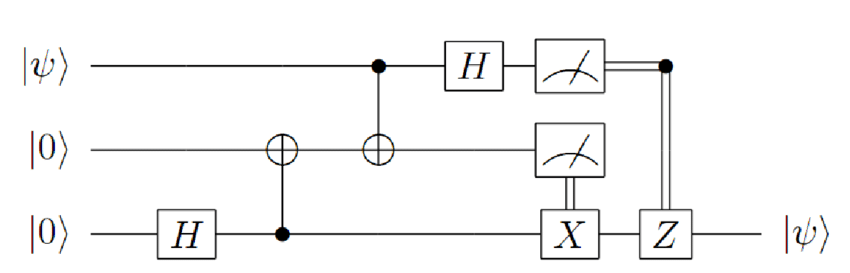
\includegraphics[width=8cm]{teleportation_circuit.png}}
\caption{Quantum Teleportation demonstrated using a quantum circuit. Input qubit $\ket{\psi}$ is transmitted to output qubit on the bottom.}
\label{teleportion}
\end{figure}

We can see in Figure \ref{teleportion} that the bottom two bits are entangled together. The top two bits are owned by the transmitter, Bob. The bottom bit is the receiver bit owned by Alice. We know from the previous section that in an entangled state, when one of the qubits is measured, both will collapse into the same state. We can express the state of the entire quantum circuit as a tensor product of each individual qubit as well as an ordered application of the quantum gates in the system.

\begin{align*}
& \text{let} \; \ket{\psi} = \begin{pmatrix}\alpha\\\beta\end{pmatrix}\\ 
& H_2C_{2,1}C_{1,0}H_1
\left [
\begin{pmatrix} \alpha \\ \beta \end{pmatrix} \otimes \begin{pmatrix} 1 \\ 0\end{pmatrix} \otimes \begin{pmatrix} 1 \\ 0\end{pmatrix}
\right ]\\
&= H_2C_{2,1}C_{1,0}
\left [
\begin{pmatrix} \alpha \\ \beta \end{pmatrix} \otimes \begin{pmatrix} \frac{1}{\sqrt{2}} \\ \frac{1}{\sqrt{2}} \end{pmatrix} \otimes \begin{pmatrix} 1 \\ 0\end{pmatrix} \right ] \; \text{$H_1$ applied}\\
&= H_2C_{2,1} \left [ \begin{pmatrix} \alpha \\ \beta \end{pmatrix} \otimes \begin{pmatrix} \frac{1}{\sqrt{2}} \\ 0 \\ 0 \\ \frac{1}{\sqrt{2}} \end{pmatrix} \right ] \; \text{$C_{1,0}$ applied}\\
&= H_2 \left [ \frac{1}{\sqrt{2}} \begin{pmatrix} \alpha \\ 0 \\ 0 \\ \alpha \\ 0 \\ \beta \\ \beta \\ 0 \end{pmatrix} \right ] = \frac{1}{2} \begin{pmatrix} \alpha \\ \beta \\ \beta \\ \alpha \\ \alpha \\ -\beta \\ -\beta \\ \alpha \end{pmatrix} \; \text{State in terms of $\ket{\psi}$}
\end{align*}

The above matrix will factor to a very interesting set sum of tensor products \cite{b9}.

\begin{gather*}
\frac{1}{2} \left ( |00\rangle \otimes \begin{bmatrix} \alpha \\ \beta \end{bmatrix}
+ |01\rangle \otimes \begin{bmatrix} \beta \\ \alpha \end{bmatrix}
+ |10\rangle \otimes \begin{bmatrix} \alpha \\ -\beta \end{bmatrix}
+ |11\rangle \otimes \begin{bmatrix} -\beta \\ \alpha \end{bmatrix} \right )
\end{gather*}

By only looking at the result above, we can see that two measured bits will tell us how the resultant teleported bit (bottom) was transmitted. Two classical bits must be transmitted to Alice to decide how to rotate her qubit. The summarize, even though it takes an infinite amount classical bits to represent any qubit state, by using entanglement, we are only required to send two classical bits to the receiver to rotate our entangled qubit after the transmitter measures the original bit on the other half of the entangled pair.

\section{Quantum Gate Algorithms}

Quantum Algorithms are usually applied to NP-Complete or NP-Hard problems where the solution to a problem is hard to find but easy to verify. Some examples may be integer factorization (basis of RSA asymmetric encryption), password cracking (one way cryptographic hash functions), unorder list sorting and more. Classical implementations of these algorithms usually employ a brute-force method in which are possible combinations are attempted. Password cracking is a great example of this with algorithms like John the Ripper which utilize a word lookup database and brute-force crack weak passwords. Quantum gate algorithms work in a completely different fashion. Most advanced quantum algorithms will take advantage of the fact that a quantum system may be initialized to hold equal probability of all $2^N$ combination of bit values. Then some operator is performed the state of the system that will amplify the ``good'' solutions.

To place the system in this state we can utilize the special properties of the Hadamard gate.

\begin{align*}
{\frac {1}{\sqrt {N}}}\sum _{x=0}^{N-1}\ket{x} =\left({\frac {1}{\sqrt {2}}}\sum _{x_{1}=0}^{1}|x_{1}\rangle \right)\otimes \cdots \otimes \left({\frac {1}{\sqrt {2}}}\sum _{x_{n}=0}^{1}\ket{x_{n}} \right)
\end{align*}

To put this in layman's terms, upon measurement, the qubits have an equal change of collapsing to any of the $2^N$ possible combinations of the binary values. To actually achieve this state we can simply clear each of the $N$ qubits to $\ket{0}$ and pass them through Hadamard gates \cite{b1}.

The next step in any quantum algorithm is to find a property of the problem we are attempting to solve and create gates that will amplify the correct states. This is known as amplitude amplification which is an entire branch of quantum computing that we will not delve into in this paper. Some interesting implementations of quantum gate algorithms include Shor's Algorithm which can factor integers in polynomial time as opposed to exponential time as seen with classical computing. Another algorithm with quantum speedup is Grover's search algorithm which can find an item in an unsorted list in $O(\sqrt{N})$ time as opposed to $O(N)$ time.

\section{Adiabatic Quantum Computing}

Adiabatic quantum computers are significantly different from the gate based quantum computer in that it can only solve a certain class of problems. This class is known as the optimization problem. A common way to visualize the optimization problem is finding the lowest point on a landscape. A more exact definition is finding the global minima inside a finite discrete function space. The conventional algorithm for this is to use the gradient descent method in which we follow the slope of the cost function down to a local minima. A quantum computer will work differently in that it operates on the property that a quantum system will naturally reach its lowest energy state under certain conditions we will discuss in a moment.

Before explaining how an adiabatic quantum computer is able to solve an optimization problem, we must first define a Hamiltonian operator. The Hamiltonian operator is a function that will compute the ``energy state'' of a given vector of inputs. The Hamiltonian will therefore define the optimization problem as a mathematical function. The classic example of the optimization problem is the traveling salesman. Here a salesman is attempting to find the best path from $A \rightarrow B$ in a weighted graph. The Hamiltonian operator will take an input vector representing a chosen path from $A \rightarrow B$ and compute the distance. This distance can be thought of as the ``energy state'' of the function at the given input vector which we are trying to minimize. The basic operating principle behind the adiabatic quantum computer is that after setting up the quantum system to model the problem's Hamiltonian operator, quantum fluctuations are applied to the system and then the system is allowed to settle \cite{b10}.

\begin{figure}[htbp]
\centerline{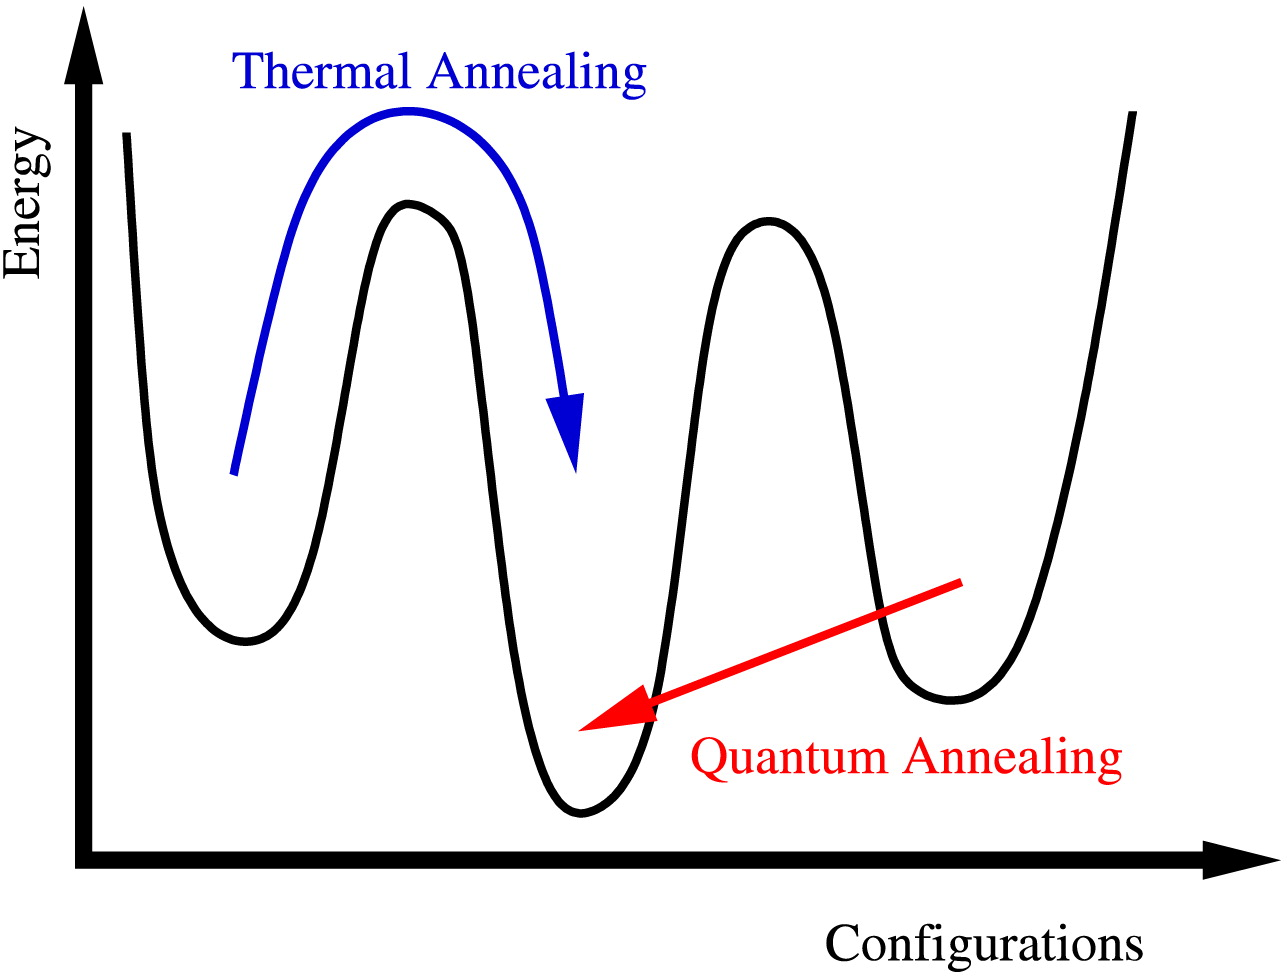
\includegraphics[width=5cm]{annealing}}
\caption{Quantum fluctuations cause the system's state to tunnel to the lowest quantum state.}
\label{annealing}
\end{figure}

The adiabatic or quantum annealing process draws from naturally occurring quantum phenomena. This phenomena is similar to the formation of diamonds or freezing of water \cite{b1}. When water is frozen slowly, perfect crystals are formed which represent the lowest energy state of system by minimizing free energy \cite{b1}. Quantum fluctuations are essentially random variations of energy at certain points in space that will cause the qubits in a quantum system to change state. Applying quantum fluctuations slowly enough so that the state of the system does not jump into an excited state is called quantum annealing.

It seems that adiabatic quantum computing has little to do with the large variety of algorithms that the gate based quantum are able to implement. However, \cite{b12} and \cite{b10} have shown that the adiabatic method is able to solve the same problems as the gate based method if a Hamiltonian operator can be extracted from the final result in the gate based algorithm. This Hamiltonian operator's ground state must have positive overlap between the lowest energy configuration and the implemented gate function. In saying this, adiabatic quantum computing is not he ``end-all'' solution to any problem. These computers are not necessarily faster than classical computing techniques for many heuristic algorithms. Adiabatic quantum computing should be limited to the problem sets that are difficult to find optimal solutions for in a classical computer. These sets of problems are called Ising problems. We can represent the Hamiltonian of an Ising problem with the following formula \cite{b13}:

\begin{align*}
{\cal H}_{ising} = & \underbrace{- \frac{A({s})}{2} \left(\sum_i {\hat\sigma_{x}^{(i)}}\right)}_\text{Initial Hamiltonian} + \\
& \underbrace{\frac{B({s})}{2} \left(\sum_{i} h_i {\hat\sigma_{z}^{(i)}} + \sum_{i>j} J_{i,j} {\hat\sigma_{z}^{(i)}} {\hat\sigma_{z}^{(j)}}\right)}_\text{Final Hamiltonian}
\end{align*}

Where ${\hat\sigma_{x,z}^{(i)}}$ are Pauli matrices operating on qubit $q_i$. $h_i$ and $J_{i,j}$ are the qubit biases and coupling strengths \cite{b13}. These biases will control how the qubits in the quantum system will interact with each other to form the Hamiltonian operator. A programmer looking to implement an adiabatic algorithm will simply need to find these coefficients of the final Hamiltonian. Once found, the Quantum Annealing process will settle the states of the qubits to the global minima of the Hamiltonian. This state will be the optimal solution to the selected problem.

\section{Implementations of Quantum Computers}

So far in this paper we have discussed the theory behind the operation of both gate based, and adiabatic quantum computers. The driving mathematics behind the operation of the quantum computer perfectly models the ideal quantum behaviour of a quantum system. In other words, this is the behaviour exhibited when the system is free from noise. To implement a qubit in real life, various methods are employed. A typical method to create a qubit is to trap an ion inside a quantum dot. Essentially this involves placing an ionized atom inside an electric field where the strength of the electric field will increase as you travel away from the center. This will trap the ion inside the center of the electric field. Two electrons from this ion are chosen to represent the qubit's quantum state. The up and down spin state of the electrons are used to represent the $\ket{0}$ and $\ket{1}$ basis vectors. Thermal energy acquired or emitted by the ion will cause the electron's state to alter which will cause the quantum system to lose coherence. To keep the ion stable, it must be cooled to millikelvin temperatures with a blue laser \cite{b1}. Quantum logic gates are done with laser or RF pulses which cause the selected electrons to change state in a predictable fashion. 

There are various other ways to represent and operate on qubits, however they all suffer from the same issues. Noise will cause the system to behave in an off-quantum way. For this reason quantum computers will often be seen in an extremely isolated environment to shield from electromagnetic and thermal radiation. The fidelity of the qubit is still a concern even at around \SI{20}{\milli\kelvin}. Quantum computers will also utilize many physical qubits to represent a single ``logical qubit''. These are called error correcting qubits and are the reason a high fidelity universal quantum computer is so hard to create.

\subsection{Real Gate Based Quantum Computers}

The private sector has taken over the quantum computing industry. IBM and Google are the leading forces in the struggle for quantum supremacy -- a goal demonstrating that a programmable quantum computer can complete a task that a classical computer cannot in a feasible amount of time \cite{b14}. While Google is quite secretive with their construction and application of their quantum computing research lab, IBM has built a 5-qubit error corrected general purpose quantum computer. It is accessible by anyone via a cloud service which will take a program written in QASM and run it on the quantum computer! This 5-qubit computer is by no means the most powerful quantum computer available today but it is one of the only gate based QCs that is available to the public. In reality, we don't need quantum computers to simulate their operation. Previous sections in this paper showed that their computational properties follow strict mathematical rules. If the quantum system is small enough (low qubit counts), we can easily simulate them using classical computers. The state vector of a 2-qubit quantum system is a $4\times 1$ vector. For every new qubit, we double the number of scalars needed to represent the qubit because the state of the system is the tensor product all of the qubit states. In November 2021, IBM revealed their new eagle processor that claims to have a 127-qubit quantum processor called the Eagle processor \cite{b15}. To be able to simulate this quantum computer with a classical one, we would need $2^{127}$ vector fields each of which fixed point fraction numbers from $0$ to $1$ in $\mathbb{C}$. We would have great difficulty running this on a conventional computer as we would need to ramp up the memory past the representable limit of 64-bit processors. Quantum Gate based technology is expected to scale up to thousands of qubits in the next couple of years which will far exceed the simulation capabilities of conventional computing. While this may sound very impressive, we are yet to see a quantum computer solve a computational problem that a conventional computer could not feasibly solve. This is mainly due to noise intruduced when performing complex algorithms such as Shor's algorithm causing the coherance of the quantum states to degrade.

\subsection{Real Adiabatic Quantum Computers}

As discussed in a previous section, adiabatic quantum computers work completely different than their gate based counterparts. For this reason their qubit counts will not compare in the same fashion as the gate based quantum computers. The only prominent company working on adiabatic QC development is a Canadian based company called D-Wave. Like IBM, D-Wave have a working quantum computer available for cloud based access to the public. D-Wave's business model is interesting in that they provide access to the quantum computer as a paid service so that other companies and researchers may run optimization problems on their machines \cite{b13}. Not only do they provide this service, D-Wave also provide an open source Python library for developing quantum algorithms that can be compiled into a Hamiltonian operator and run on adiabatic hardware.

\begin{figure}[htbp]
\centerline{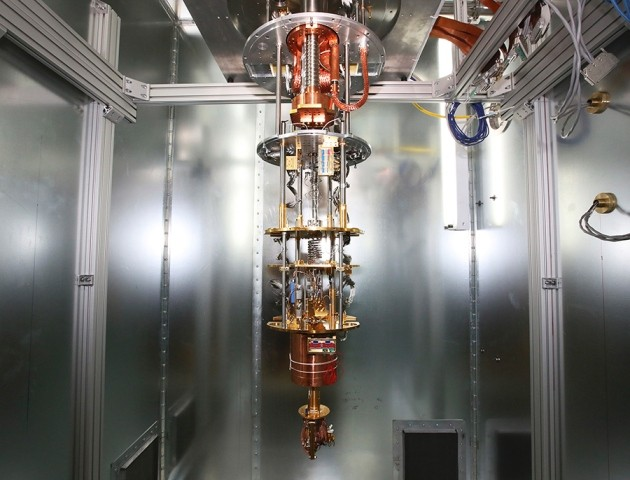
\includegraphics[width=6cm]{dwave}}
\caption{D-Wave's Adiabatic Quantum Computer inside a cryogenic dilution chamber to shield against thermal and electromagnetic noise.}
\label{dwave}
\end{figure}

An interesting bonus of quantum computing is that because the computer's state is represented by natural quantum phenomena, the actual power usage of the quantum computer is extremely low (not measurable) \cite{b13}. Essentially all of the power usage of the quantum computer comes from cooling the processor down to cryogenic temperatures to shield the qubits from as much noise as possible.

\section{Conclusion}

While quantum computing will impact society in the future, it has not yet reached the scale needed for medium and small companies to own and operate one. Over the next couple of years, we will most likely see quantum compute power rented out to licensed users by large companies like Microsoft Azure Quantum, Amazon Braket and IBM  \cite{b1}. Quantum speedup of computationally intensive algorithms will help with many fields including physics, medical, financial and especially computer science. \cite{b2} claims that the applications of quantum computing is currently difficult to classify as we won't know until they become readily available.

Quantum Computing skeptics such as \cite{b16} claim that as quantum computing scales to large sizes, amount of error correction required to keep the quantum system at high fidelity would not be feasible as adding more qubits to the quantum system can bog it down with additional noise. \cite{b16} also claims that the noise introduced by new qubits to the system would cause the coherence of the quantum system to degrade past the point of usability.

Regardless of whether or not a high fidelity universal quantum computer is feasible, this field provides a very interesting branch of computer architecture and design that will undoubtedly impact our lives in some way in the near future.

\begin{thebibliography}{00}
\bibitem{b1} V. Kasirajan, Fundamentals of quantum computing: Theory and practice. S.l.: Springer, 2021.
\bibitem{b2} “Quantum Computing - IOPscience - Institute of Physics,” 13-Aug-1997. [Online]. Available: https://iopscience.iop.org/article/10.1088/0034-4885/61/2/002. [Accessed: 04-Dec-2021]. 
\bibitem{b3} M. Sparkes, “IBM creates largest ever superconducting quantum computer,” New Scientist, 18-Nov-2021. [Online]. Available: https://www.newscientist.com/article/2297583-ibm-creates-largest-ever-superconducting-quantum-computer/. [Accessed: 04-Dec-2021]. 
\bibitem{b4} P. Ball, “Two slits and one hell of a quantum conundrum,” Nature News, 07-Aug-2018. [Online]. Available: https://www.nature.com/articles/d41586-018-05892-6. [Accessed: 04-Dec-2021].
\bibitem{b5} A. Dawar, “What is quantum computing?” [Online]. Available: https://www.cl.cam.ac.uk/teaching/0910/QuantComp/notes.pdf. [Accessed: 04-Dec-2021].
\bibitem{b6} O. Titiloye and A. Crispin, “Quantum annealing of the graph coloring problem,” Discrete Optimization, vol. 8, no. 2, pp. 376–384, 2011. 
\bibitem{b7} S. Takeda, T. Mizuta, M. Fuwa, P. van Loock, and A. Furusawa, “Deterministic quantum teleportation of photonic quantum bits by a hybrid technique,” Nature News, 14-Aug-2013. [Online]. Available: https://www.nature.com/articles/nature12366/. [Accessed: 06-Dec-2021]. 
\bibitem{b8} V. Vedral, “Quantum Entanglement,” Nature News, 01-Apr-2014. [Online]. Available: https://www.nature.com/articles/nphys2904. [Accessed: 06-Dec-2021]. 
\bibitem{b9} Nillmer, “Building a matrix corresponding to the teleportation circuit,” Quantum Computing Stack Exchange, 13-Dec-2018. [Online]. Available: https://quantumcomputing.stackexchange.com/questions/4917/building-a-matrix-corresponding-to-the-teleportation-circuit. [Accessed: 06-Dec-2021].
\bibitem{b10} P. Ray, B. K. Chakrabarti, and A. Chakrabarti, “Sherrington-Kirkpatrick model in a transverse field: Absence of replica symmetry breaking due to quantum fluctuations,” Physical Review B, 01-Jun-1989. [Online]. Available: https://doi.org/10.1103/PhysRevB.39.11828. [Accessed: 06-Dec-2021]. 
\bibitem{b11} V. Bapst, L. Foini, F. Krzakala, G. Semerjian, and F. Zamponi, “The quantum adiabatic algorithm applied to random optimization problems: The Quantum Spin Glass Perspective,” Physics Reports, vol. 523, no. 3, pp. 127–205, 2013.
\bibitem{b12} D. Aharonov, D. Gottesman, S. Irani, and J. Kempe, “The power of quantum systems on a line,” Communications in Mathematical Physics, 13-Jan-2009. [Online]. Available: https://link.springer.com/article/10.1007/s00220-008-0710-3. [Accessed: 06-Dec-2021]. 
\bibitem{b13} “What is quantum annealing?.” [Online]. Available: https://docs.dwavesys.com/docs/latest/c\_gs\_2.html. [Accessed: 06-Dec-2021]. 
\bibitem{b14} J. Preskill, “Quantum Computing in the NISQ era and beyond,” Quantum, 06-Aug-2018. [Online]. Available: https://doi.org/10.22331/q-2018-08-06-79. [Accessed: 06-Dec-2021].
\bibitem{b15} “IBM unveils breakthrough 127-qubit quantum processor,” IBM Newsroom. [Online]. Available: https://newsroom.ibm.com/2021-11-16-IBM-Unveils-Breakthrough-127-Qubit-Quantum-Processor. [Accessed: 06-Dec-2021]. 
\bibitem{b16} D. Aharonov, M. Ben-Or, R. Impagliazzo, and N. Nisan, “[PDF] limitations of noisy reversible computation: Semantic scholar,” undefined, 01-Jan-1996. [Online]. Available: https://www.semanticscholar.org/paper/Limitations-of-Noisy-Reversible-Computation-Aharonov-Ben-Or/658ce5e47e404ea30fdb671a514b6cc293122685. [Accessed: 06-Dec-2021]. 
\end{thebibliography}

\end{document}
